\documentclass{beamer}

\usepackage{graphicx}
\usepackage{textpos}
\usepackage{listings}
\usepackage{lstautogobble}

\usetheme{Madrid}
\useoutertheme{miniframes} % Alternatively: miniframes, infolines, split

% Setup the university's color pallette
\definecolor{UIUCorange}{RGB}{19, 41, 75} % UBC Blue (primary)
\definecolor{UIUCblue}{RGB}{232, 74, 39} % UBC Grey (secondary)

\definecolor{codegreen}{rgb}{0,0.6,0}
\definecolor{codegray}{rgb}{0.5,0.5,0.5}
\definecolor{codepurple}{rgb}{0.58,0,0.82}
\definecolor{backcolour}{rgb}{0.95,0.95,0.92}

\lstdefinestyle{python}{
  backgroundcolor=\color{backcolour},   
  commentstyle=\color{codegreen},
  keywordstyle=\color{magenta},
  numberstyle=\tiny\color{codegray},
  stringstyle=\color{codepurple},
  basicstyle=\ttfamily\footnotesize,
  breakatwhitespace=false,         
  belowskip=-0.5em,
  breaklines=true,                 
  captionpos=b,                    
  keepspaces=true,                 
  numbers=left,                    
  numbersep=5pt,                  
  showspaces=false,                
  showstringspaces=false,
  showtabs=false,                  
  tabsize=2
}

\lstset{style=python}

\AtBeginSection[]{
    \begin{frame}
        \vfill
        \centering
        \begin{beamercolorbox}[sep=8pt,center,shadow=true,rounded=true]{title}
            \usebeamerfont{title}\insertsectionhead\par%
        \end{beamercolorbox}
        \vfill
    \end{frame}
}
% Setup the university's color pallette
\definecolor{UIUCorange}{RGB}{19, 41, 75} % UBC Blue (primary)
\definecolor{UIUCblue}{RGB}{232, 74, 39} % UBC Grey (secondary)


\setbeamercolor{palette primary}{bg=UIUCorange,fg=white}
\setbeamercolor{palette secondary}{bg=UIUCblue,fg=white}
\setbeamercolor{palette tertiary}{bg=UIUCblue,fg=white}
\setbeamercolor{palette quaternary}{bg=UIUCblue,fg=white}
\setbeamercolor{structure}{fg=UIUCorange} % itemize, enumerate, etc
\setbeamercolor{section in toc}{fg=UIUCblue} % TOC sections

\setbeamercolor{subsection in head/foot}{bg=UIUCorange,fg=UIUCblue}
\setbeamercolor{subsection in head/foot}{bg=UIUCorange,fg=UIUCblue}

\usepackage[utf8]{inputenc}
\usepackage{graphicx}

%Information to be included in the title page:
\title{\textbf{Adv. Strings}}
\author{\textbf{David H Smith IV}}
\institute[\textbf{UIUC}]{\textbf{University of Illinois Urbana-Champaign}}
\date{\textbf{Tues, Oct 4 2021}}

\setbeamertemplate{title page}[default][colsep=-4bp,rounded=true]
\addtobeamertemplate{title page}{\vspace{3\baselineskip}}{}
\addtobeamertemplate{title page}{
  \begin{textblock*}{\paperwidth}(-1.0em, -1.2em)
    
\includegraphics[width=\paperwidth, height=\paperheight]{imgs/uiuc.png}
  \end{textblock*} 
}{}

\begin{document}

\frame{\titlepage}

\section{Reminders}

%
% Slide 1
%
\begin{frame}
  \frametitle{Reminders}
  \begin{itemize}
    \item Post-reading 9p1 is due Tommorow (will be posted after class).
    \item Homework 8 is due tommorow.
    \item Participation 9p1 is due Tommorow.
    \item Lab 4 is due Sunday after next.
  \end{itemize}
\end{frame}

\section{Strings Slicing}


%
% Slide 2
%
\begin{frame}[fragile]
  \frametitle{Poll Question: Slicing}
  What is the result of running this code?
  \begin{lstlisting}[language=Python, autogobble]
  my_str = "CS 105"
  print(my_str[1:2])
  \end{lstlisting}
  \vfill
  \begin{enumerate}[A]
    \item \lstinline|'C'|
    \item \lstinline|'CS'|
    \item \lstinline|'CS '|
    \item \lstinline|'S'|
    \item \lstinline|'S '|
  \end{enumerate}
\end{frame}



%
% Slide 2
%
\begin{frame}[fragile]
  \frametitle{Poll Question: Slicing}
  What is the result of running this code?
  \begin{lstlisting}[language=Python, autogobble]
  my_str = "CS 105"
  print(my_str[-4:-2])
  \end{lstlisting}
  \vfill
  \begin{enumerate}[A]
    \item \lstinline|'S 1'|
    \item \lstinline|'S 10'|
    \item \lstinline|' 1'|
    \item \lstinline|' 10'|
  \end{enumerate}
\end{frame}



%
% Slide 2
%
\begin{frame}[fragile]
  \frametitle{Poll Question: Slicing}
  What is the result of running this code?
  \begin{lstlisting}[language=Python, autogobble]
  my_str = "CS 105"
  print(my_str([::2]))
  \end{lstlisting}
  \vfill
  \begin{enumerate}[A]
    \item \lstinline|'C'|
    \item \lstinline|'CS'|
    \item \lstinline|'S'|
    \item \lstinline|'C 0'|
  \end{enumerate}
\end{frame}


%
% Slide 2
%
\begin{frame}[fragile]
  \frametitle{Slicing}
  \begin{enumerate}[A]
    \item \lstinline|string[start:stop:interval]|
    \item Like range, start is inclusive stop is exclusive.
    \item Interval default is 1
    \item Interval is optional
  \end{enumerate}
\end{frame}

\section{Split}

%
% Slide 2
%
\begin{frame}[fragile]
  \frametitle{Poll Question: Splitting}
  What is the result of running this code?
  \begin{lstlisting}[language=Python, autogobble]
  my_str = "CS 105 rox"
  result = my_str.split()
  \end{lstlisting}
  \vfill
  \begin{enumerate}[A]
    \item \lstinline|("CS", "105", "rox")|
    \item \lstinline|["CS 105 rox"]|
    \item \lstinline|["CS", "105 rox"]|
    \item \lstinline|["CS", "105", "rox"]|
  \end{enumerate}
\end{frame}



%
% Slide 2
%
\begin{frame}[fragile]
  \frametitle{Poll Question: Splitting}
  What is the result of running this code?
  \begin{lstlisting}[language=Python, autogobble]
  csv = "1, 2, 3, 4"
  result = csv.split(",")
  \end{lstlisting}
  \vfill
  \begin{enumerate}[A]
    \item \lstinline|['1']|
    \item \lstinline|['1, 2, 3, 4']|
    \item \lstinline|['1', ' 2', ' 3', ' 4']|
    \item \lstinline|['1,', '2,', '3,', '4']|
  \end{enumerate}
\end{frame}


\section{Join}

%
% Slide 2
%
\begin{frame}[fragile]
  \frametitle{Poll Question: Joining}
  What is the result of running this code?
  \begin{lstlisting}[language=Python, autogobble]
  numlist = [1, 2, 3, 4]
  result = ",".join(numlist)
  \end{lstlisting}
  \vfill
  \begin{enumerate}[A]
    \item \lstinline|'1234'|
    \item \lstinline|'1,2,3,4'|
    \item \lstinline|'1, 2, 3, 4'|
    \item \lstinline|TypeError|
  \end{enumerate}
  \pause
  How do we fix this?
\end{frame}


%
% Slide 2
%
\begin{frame}[fragile]
  \frametitle{A Common Pattern}
  The generic pattern:
  \begin{lstlisting}[language=Python, autogobble]
  mylist = input_data.split(<separator>)
  ... data processing ...
  outputstring "<separator>".join(my_list)
  \end{lstlisting}
  \vfill
  An example of this being done on one line:
  \begin{lstlisting}[language=Python, autogobble]
  output = ",".join(string.split(",")[::2])
  \end{lstlisting}
\end{frame}


%
% Slide 2
%
\begin{frame}[fragile]
  \frametitle{Pattern Practice}
  Write some code that takes a string with comma separated integers
  that converts the string into the square of each original value.
  \vfill
  \textbf{Go to PrairieLearn to do this problem}
\end{frame}

%
% Slide 2
%
\begin{frame}[fragile]
  \frametitle{Pattern Practice}
  \begin{lstlisting}[language=Python, autogobble]
  def foo(numlist):
    squaredlist = []
    for num in numlist.split(","):
      squaredlist.append(str(int(num) ** 2))
    return ",".join(squaredlist)
  \end{lstlisting}
\end{frame}

\section{Adv. String Formatting}

%
% Slide 2
%
\begin{frame}[fragile]
  \frametitle{Adv. String Formatting}
	\begin{figure}
		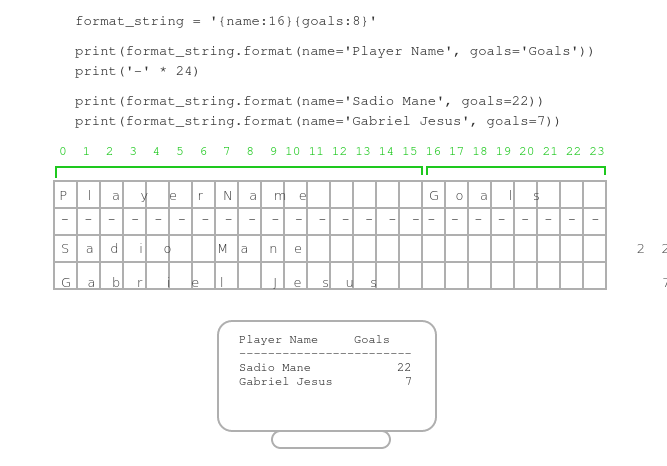
\includegraphics[width=\textwidth]{./imgs/width.png}
	\end{figure}
\end{frame}

%
% Slide 2
%
\begin{frame}[fragile]
  \frametitle{Alignment}
  For a field width of 10:
  \begin{enumerate}
    \item \textbf{Left-aligned: } \lstinline|"{:<10}".format(x)|
    \item \textbf{Right-aligned: } \lstinline|"{:>10}".format(x)|
    \item \textbf{Centered: } \lstinline|"{:^10}".format(x)|
  \end{enumerate}
  \vfill
  Notice the similarity between field width and how we set the number of decimals after a floating point: \lstinline|"{:.2f}".format(math.pi)| \textrightarrow $3.14$.
  \pause
  \vfill
  We can use a fill character to consume any unused spaces in the field width:
  \begin{enumerate}
    \item \textbf{Left-aligned: } \lstinline|"{:-<10}".format(x)|
    \item \textbf{Right-aligned: } \lstinline|"{:->10}".format(x)|
    \item \textbf{Centered: } \lstinline|"{:-^10}".format(x)|
  \end{enumerate}
\end{frame}

\begin{frame}[fragile]
  \frametitle{Formatting Practice}
	Create a function that takes a list of lists where each sub list contains 4
	elements. Create and return a new list of strings where each string is composed
	of the four elements in each sublist and:
	\begin{enumerate}
		\item the first element is center aligned with a field with of 10
		\item the second element is right aligned with a field width of 8
		\item the third element is left aligned with a field width of 9
		\item the fourth element is center aligned with a field width of 10 and the filler character "-".
	\end{enumerate}
	\textbf{Problem is on PrairieLearn}
\end{frame}

%
% Slide 2
%
\begin{frame}[fragile]
  \frametitle{Example Function Call}
  \begin{lstlisting}[language=Python, autogobble]
	x = [
		["This", "is", "a", "list"],
		["This", "is", "a", "list"],
		["This", "is", "a", "list"],
		["This", "is", "a", "list"],
		["This", "is", "a", "list"],
		["This", "is", "a", "list"],
		["This", "is", "a", "list"],
		["This", "is", "a", "list"],
    ...
	]
	formatted_x = formatted_str_list(x)
  \end{lstlisting}
\end{frame}


%
% Slide 2
%
\begin{frame}[fragile]
  \frametitle{Pattern Practice}
  \begin{lstlisting}[language=Python, autogobble]
	def formatted_str_list(x):
		formatted_strs = []
		for a, b, c, d in x:
			y = "{:^10}{:>8}{:<9}{:-^10}".format(a, b, c, d)
			formatted_strs.append(y)
		return formatted_strs

	x = [
		["This", "is", "a", "list"],
		["This", "is", "a", "list"],
		["This", "is", "a", "list"],
		["This", "is", "a", "list"]
	]
	formatted_x = formatted_str_list(x)
  \end{lstlisting}
\end{frame}

\section{Patterns (Part 1)}

%
% Slide 2
%
\begin{frame}[fragile]
  \frametitle{Counting Pattern}
  \begin{lstlisting}[language=Python, autogobble][language=Python, autogobble]
  def count(collection):
    counter = 0
    for item in collection:
      if <item meets condition>:
        counter += 1
    return counter
  \end{lstlisting}
\end{frame}

%
% Slide 2
%
\begin{frame}[fragile]
  \frametitle{Computing a Sum/Total}
  \begin{lstlisting}[language=Python, autogobble][language=Python, autogobble]
  def sum(collection):
    total = 0
    for item in collection:
      total += item
    return total
  \end{lstlisting}
\end{frame}


%
% Slide 2
%
\begin{frame}[fragile]
  \frametitle{Pattern Practice}
  Spend remaining class time working on last three problems in PrairieLearn.
\end{frame}

\end{document}
